\documentclass[11pt]{article}
\usepackage{amsmath}
\usepackage{amsfonts}
\usepackage{graphicx}
\usepackage[margin = 1.2 in]{geometry}
\usepackage{pgfplots}
\usepackage{tikz}
\usepackage[siunitx]{circuitikz}
\usepackage[makeroom]{cancel}

%opening
\title{Ohm's and Kirchoff's Laws}
\author{Andreas Badea}
\date{February 7, 2018}
\begin{filecontents*}{data2.csv}
	res3t,res3v,res3i,res2t,res2v,res2i,lit,liv,lii,res1t,res1v,res1i
	0,-0.00152587890625,-0.0006103515625,0,-0.001220703125,-7.62939453125E-05,0,-0.023193359375,0.00137329101563,0,0.0018310546875,-5.72204589844E-05
	0.666666666667,0.00732421875,0.000114440917969,0.666666666667,-0.0006103515625,-3.81469726563E-05,0.666666666667,-0.0228881835938,0.00131607055664,0.666666666667,0.00213623046875,-7.62939453125E-05
	1.33333333333,-0.003662109375,0.000324249267578,1.33333333333,-0.0006103515625,-3.81469726563E-05,1.33333333333,-0.0225830078125,0.0013542175293,1.33333333333,0.00244140625,-7.62939453125E-05
	2,0.0018310546875,0.000267028808594,2,-0.0006103515625,-7.62939453125E-05,2,-0.0228881835938,0.00139236450195,2,0.0018310546875,-7.62939453125E-05
	2.66666666667,0.0213623046875,0.000381469726563,2.66666666667,0,-5.72204589844E-05,2.66666666667,-0.023193359375,0.0013542175293,2.66666666667,0.00213623046875,-7.62939453125E-05
	3.33333333334,0.0265502929688,0.000381469726563,3.33333333333,0,-0.000114440917969,3.33333333333,-0.0222778320313,0.00137329101563,3.33333333334,0.00244140625,-5.72204589844E-05
	4,0.0393676757813,-0.000209808349609,4,-0.00030517578125,-0.000114440917969,4,-0.023193359375,0.00139236450195,4,0.00244140625,-7.62939453125E-05
	4.66666666667,0.0213623046875,0.000267028808594,4.66666666667,-0.0006103515625,-5.72204589844E-05,4.66666666667,-0.0222778320313,0.0013542175293,4.66666666667,0.0018310546875,-9.53674316406E-05
	5.33333333334,0.0274658203125,-0.000343322753906,5.33333333333,-0.001220703125,-7.62939453125E-05,5.33333333333,-0.023193359375,0.00139236450195,5.33333333334,0.00213623046875,-9.53674316406E-05
	6,0.182800292969,0.000400543212891,6,-0.00030517578125,-0.000114440917969,6,-0.023193359375,0.00154495239258,6,0.0018310546875,-5.72204589844E-05
	6.66666666667,0.253295898438,-0.000209808349609,6.66666666667,-0.00030517578125,-9.53674316406E-05,6.66666666667,-0.02197265625,0.00158309936523,6.66666666667,0.00244140625,-9.53674316406E-05
	7.33333333334,0.340270996094,0.000171661376953,7.33333333333,0.0006103515625,-9.53674316406E-05,7.33333333333,0.00152587890625,0.0123977661133,7.33333333334,0.00213623046875,-7.62939453125E-05
	8,0.508728027344,0.000495910644531,8,-0.00030517578125,-0.000114440917969,8,-0.001220703125,0.0105094909668,8,0.00244140625,-7.62939453125E-05
	8.66666666667,0.513610839844,-0.000457763671875,8.66666666667,-0.00030517578125,-5.72204589844E-05,8.66666666667,0.00152587890625,0.0118446350098,8.66666666667,0.00274658203125,-7.62939453125E-05
	9.33333333334,0.712890625,0.000495910644531,9.33333333333,0,-0.000114440917969,9.33333333333,0.0048828125,0.0134658813477,9.33333333334,0.025634765625,0
	10,0.704345703125,-0.000247955322266,10,0.0006103515625,-0.000152587890625,10,0.167846679688,0.0868797302246,10,0.0289916992188,0
	10.6666666667,0.4443359375,0,10.6666666667,0,-9.53674316406E-05,10.6666666667,0.238647460938,0.113945007324,10.6666666667,0.0302124023438,-1.90734863281E-05
	11.3333333333,0.431823730469,0.000514984130859,11.3333333333,0.0112915039063,-7.62939453125E-05,11.3333333333,0.314636230469,0.140171051025,11.3333333333,0.0296020507813,-1.90734863281E-05
	12,0.403137207031,-0.000457763671875,12,0.230712890625,3.81469726563E-05,12,0.432739257813,0.171165466309,12,0.0341796875,-1.90734863281E-05
	12.6666666667,0.557250976563,0.000267028808594,12.6666666667,0.335388183594,5.72204589844E-05,12.6666666667,0.624694824219,0.184593200684,12.6666666667,0.145568847656,0.000228881835938
	13.3333333333,0.609130859375,-0.00030517578125,13.3333333333,0.330505371094,9.53674316406E-05,13.3333333333,0.76904296875,0.187644958496,13.3333333333,0.27099609375,0.000400543212891
	14,0.698852539063,0.000476837158203,14,0.378723144531,9.53674316406E-05,14,0.833435058594,0.192050933838,14,0.387878417969,0.0006103515625
	14.6666666667,0.787658691406,0.000114440917969,14.6666666667,0.823974609375,0.000209808349609,14.6666666667,0.902709960938,0.197143554688,14.6666666667,0.390319824219,0.000648498535156
	15.3333333333,0.797424316406,0,15.3333333333,0.835266113281,0.000228881835938,15.3333333333,1.02355957031,0.208320617676,15.3333333333,0.504455566406,0.000839233398438
	16,0.88134765625,0.000286102294922,16,0.841369628906,0.000228881835938,16,1.12823486328,0.21484375,16,0.507507324219,0.000896453857422
	16.6666666667,0.921325683594,3.81469726563E-05,16.6666666667,1.26586914063,0.000362396240234,16.6666666667,1.26373291016,0.226402282715,16.6666666667,0.632019042969,0.00101089477539
	17.3333333333,0.935668945313,1.90734863281E-05,17.3333333333,1.41937255859,0.000438690185547,17.3333333333,1.4453125,0.240821838379,17.3333333333,0.717468261719,0.00127792358398
	18,0.929870605469,0.00030517578125,18,1.41937255859,0.000457763671875,18,1.56311035156,0.249214172363,18,0.831604003906,0.00137329101563
	18.6666666667,1.00708007813,0.000114440917969,18.6666666667,1.53472900391,0.000476837158203,18.6666666667,1.71600341797,0.260562896729,18.6666666667,0.874328613281,0.00146865844727
	19.3333333333,1.07086181641,0.000343322753906,19.3333333333,1.56402587891,0.000495910644531,19.3333333333,1.71783447266,0.260677337646,19.3333333333,0.886535644531,0.00148773193359
	20,1.09436035156,0.000343322753906,20,1.66748046875,0.000514984130859,20,1.90979003906,0.274906158447,20,1.01257324219,0.00179290771484
	20.6666666667,1.13800048828,0.000152587890625,20.6666666667,1.66900634766,0.000495910644531,20.6666666667,1.89910888672,0.274085998535,20.6666666667,1.17492675781,0.00211715698242
	21.3333333333,1.19323730469,0.000209808349609,21.3333333333,1.81488037109,0.0006103515625,21.3333333333,2.07458496094,0.286083221436,21.3333333333,1.24084472656,0.00228881835938
	22,1.21459960938,0.000324249267578,22,1.92077636719,0.000572204589844,22,2.20062255859,0.29504776001,22,1.24420166016,0.00232696533203
	22.6666666667,1.26312255859,0.000286102294922,22.6666666667,1.91467285156,0.0006103515625,22.6666666667,2.29248046875,0.30101776123,22.6666666667,1.24877929688,0.00228881835938
	23.3333333333,1.3720703125,0.000267028808594,23.3333333333,2.05596923828,0.000667572021484,23.3333333333,2.431640625,0.309925079346,23.3333333333,1.32385253906,0.00238418579102
	24,1.39678955078,0.000267028808594,24,2.22320556641,0.000743865966797,24,2.52777099609,0.315856933594,24,1.37512207031,0.00247955322266
	24.6666666667,1.48010253906,0.00030517578125,24.6666666667,2.236328125,0.000724792480469,24.6666666667,2.54089355469,0.316581726074,24.6666666667,1.43432617188,0.00255584716797
	25.3333333333,1.552734375,0.000324249267578,25.3333333333,2.37701416016,0.000820159912109,25.3333333333,2.51220703125,0.314483642578,25.3333333333,1.48986816406,0.00272750854492
	26,1.69067382813,0.000381469726563,26,2.49847412109,0.000858306884766,26,2.37915039063,0.306377410889,26,1.58355712891,0.00278472900391
	26.6666666667,1.78894042969,0.000228881835938,26.6666666667,2.54333496094,0.000820159912109,26.6666666667,2.34771728516,0.304393768311,26.6666666667,1.58386230469,0.00295639038086
	27.3333333333,1.79046630859,0.000381469726563,27.3333333333,2.57110595703,0.000858306884766,27.3333333333,2.29187011719,0.300731658936,27.3333333333,1.57745361328,0.00274658203125
	28,1.90795898438,0.000381469726563,28,2.79602050781,0.000953674316406,28,2.24426269531,0.297031402588,28,1.60888671875,0.00289916992188
	28.6666666667,1.9921875,0.000419616699219,28.6666666667,2.87384033203,0.000991821289063,28.6666666667,2.16583251953,0.291919708252,28.6666666667,1.69494628906,0.00297546386719
	29.3333333333,2.06817626953,0.000438690185547,29.3333333333,2.90130615234,0.000991821289063,29.3333333333,2.16217041016,0.291709899902,29.3333333333,1.76239013672,0.0031852722168
	30,2.13989257813,0.000419616699219,30,3.17138671875,0.00104904174805,30,2.07885742188,0.285415649414,30,1.89605712891,0.00329971313477
	30.6666666667,2.1484375,0.000362396240234,30.6666666667,3.17199707031,0.00112533569336,30.6666666667,1.98181152344,0.278968811035,30.6666666667,1.90246582031,0.00347137451172
	31.3333333333,2.21252441406,0.000362396240234,31.3333333333,3.45733642578,0.00131607055664,31.3333333333,1.96899414063,0.277938842773,31.3333333333,1.98516845703,0.00345230102539
	32,2.30133056641,0.000476837158203,32,3.60778808594,0.00133514404297,32,1.85363769531,0.270099639893,32,2.10052490234,0.00377655029297
	32.6666666667,2.31628417969,0.000419616699219,32.6666666667,3.61755371094,0.0013542175293,32.6666666667,1.8212890625,0.267524719238,32.6666666667,2.22015380859,0.00396728515625
	33.3333333333,2.40142822266,0.000514984130859,33.3333333333,3.61602783203,0.00133514404297,33.3333333333,1.73583984375,0.260772705078,33.3333333333,2.25372314453,0.00404357910156
	34,2.42279052734,0.000553131103516,34,3.77777099609,0.00131607055664,34,1.66015625,0.254688262939,34,2.30682373047,0.00417709350586
	34.6666666667,2.42523193359,0.000534057617188,34.6666666667,3.89434814453,0.00131607055664,34.6666666667,1.60369873047,0.250205993652,34.6666666667,2.35046386719,0.0042724609375
	35.3333333334,2.43499755859,0.000534057617188,35.3333333333,3.95690917969,0.00141143798828,35.3333333333,1.58935546875,0.24959564209,35.3333333334,2.40753173828,0.00431060791016
	36,2.55554199219,0.000572204589844,36,3.98345947266,0.00143051147461,36,1.49810791016,0.242385864258,36,2.42279052734,0.00432968139648
	36.6666666667,2.60406494141,0.000476837158203,36.6666666667,4.14154052734,0.00144958496094,36.6666666667,1.48590087891,0.241546630859,36.6666666667,2.48931884766,0.00444412231445
	37.3333333334,2.67181396484,0.000572204589844,37.3333333333,4.18182373047,0.00144958496094,37.3333333333,1.44866943359,0.238819122314,37.3333333334,2.70599365234,0.00503540039063
	38,2.72399902344,0.000514984130859,38,4.19372558594,0.00144958496094,38,1.37725830078,0.232715606689,38,2.83477783203,0.00513076782227
	38.6666666667,2.78533935547,0.000534057617188,38.6666666667,4.22637939453,0.00143051147461,38.6666666667,1.25396728516,0.2219581604,38.6666666667,2.82745361328,0.00513076782227
	39.3333333334,2.83538818359,0.000572204589844,39.3333333333,4.44396972656,0.00156402587891,39.3333333333,1.15692138672,0.213756561279,39.3333333334,2.83264160156,0.00516891479492
	40,2.94128417969,0.000572204589844,40,4.54284667969,0.00158309936523,40,1.11145019531,0.210037231445,40,2.83233642578,0.00497817993164
	40.6666666667,2.96203613281,0.000553131103516,40.6666666667,4.72869873047,0.00167846679688,40.6666666667,1.0595703125,0.205955505371,40.6666666667,2.83813476563,0.00514984130859
	41.3333333334,3.09265136719,0.0006103515625,41.3333333333,4.98474121094,0.00181198120117,41.3333333333,0.96435546875,0.197448730469,41.3333333334,2.86560058594,0.0050163269043
	42,3.11187744141,0.000591278076172,42,4.97772216797,0.0018310546875,42,0.928344726563,0.193824768066,42,2.89428710938,0.00516891479492
	42.6666666667,3.22479248047,0.000629425048828,42.6666666667,4.97436523438,0.0018310546875,42.6666666667,0.871276855469,0.189552307129,42.6666666667,3.00598144531,0.00534057617188
	43.3333333334,3.27758789063,0.000629425048828,43.3333333333,4.74609375,0.00165939331055,43.3333333333,0.809631347656,0.181713104248,43.3333333334,3.06915283203,0.00579833984375
	44,3.32855224609,0.0006103515625,44,4.52911376953,0.00160217285156,44,0.751342773438,0.177001953125,44,3.19488525391,0.00576019287109
	44.6666666667,3.41430664063,0.000686645507813,44.6666666667,4.51293945313,0.00158309936523,44.6666666667,0.707397460938,0.174903869629,44.6666666667,3.22021484375,0.00587463378906
	45.3333333334,3.46771240234,0.000648498535156,45.3333333333,4.43603515625,0.00150680541992,45.3333333333,0.638122558594,0.169372558594,45.3333333334,3.26354980469,0.00577926635742
	46,3.4716796875,0.000686645507813,46,4.37072753906,0.00150680541992,46,0.604858398438,0.166854858398,46,3.40728759766,0.00591278076172
	46.6666666667,3.51409912109,0.000648498535156,46.6666666667,4.37103271484,0.00156402587891,46.6666666667,0.533752441406,0.159492492676,46.6666666667,3.42834472656,0.00593185424805
	47.3333333334,3.56018066406,0.000686645507813,47.3333333333,4.30084228516,0.00144958496094,47.3333333333,0.488891601563,0.155639648438,47.3333333334,3.49395751953,0.00635147094727
	48,3.71215820313,0.000686645507813,48,4.15679931641,0.00146865844727,48,0.405883789063,0.138339996338,48,3.64868164063,0.00663757324219
	48.6666666667,3.71429443359,0.000686645507813,48.6666666667,4.05975341797,0.00143051147461,48.6666666667,0.397033691406,0.145664215088,48.6666666667,3.71887207031,0.00661849975586
	49.3333333334,3.72192382813,0.000705718994141,49.3333333333,3.98529052734,0.0013542175293,49.3333333333,0.340881347656,0.133724212646,49.3333333334,3.828125,0.00699996948242
	50,3.81774902344,0.000743865966797,50,3.84490966797,0.00141143798828,50,0.276489257813,0.117950439453,50,3.96606445313,0.00696182250977
	50.6666666667,3.85681152344,0.000743865966797,50.6666666667,3.83270263672,0.00137329101563,50.6666666667,0.21728515625,0.100574493408,50.6666666667,4.06402587891,0.00736236572266
	51.3333333334,4.03137207031,0.000820159912109,51.3333333333,3.79333496094,0.00139236450195,51.3333333333,0.203247070313,0.0966262817383,51.3333333334,4.19219970703,0.00747680664063
	52,4.04205322266,0.000801086425781,52,3.50036621094,0.00123977661133,52,0.0250244140625,0.0222015380859,52,4.27185058594,0.00753402709961
	52.6666666667,4.17663574219,0.000839233398438,52.6666666667,3.37615966797,0.00114440917969,52.6666666667,0.0100708007813,0.0161170959473,52.6666666667,4.38232421875,0.0078010559082
	53.3333333334,4.21295166016,0.000801086425781,53.3333333333,3.30505371094,0.00116348266602,53.3333333333,0.00579833984375,0.0138664245605,53.3333333334,4.46838378906,0.00820159912109
	54,4.25903320313,0.000801086425781,54,3.11553955078,0.0010871887207,54,-0.0228881835938,0.00143051147461,54,4.63317871094,0.00825881958008
	54.6666666667,4.32800292969,0.000858306884766,54.6666666667,3.02551269531,0.00101089477539,54.6666666667,-0.02197265625,0.0013542175293,54.6666666667,4.66613769531,0.00846862792969
	55.3333333334,4.35272216797,0.000839233398438,55.3333333333,2.87963867188,0.000972747802734,55.3333333333,-0.0225830078125,0.00131607055664,55.3333333334,4.74182128906,0.00871658325195
	56,4.42718505859,0.000858306884766,56,2.8564453125,0.00102996826172,56,-0.02197265625,0.00131607055664,56,4.80651855469,0.00875473022461
	56.6666666667,4.44396972656,0.000934600830078,56.6666666667,2.74536132813,0.00091552734375,56.6666666667,-0.0222778320313,0.00131607055664,56.6666666667,4.92156982422,0.00892639160156
	57.3333333334,4.50378417969,0.000877380371094,57.3333333333,2.54760742188,0.000820159912109,57.3333333333,-0.0222778320313,0.0013542175293,57.3333333334,4.96032714844,0.00909805297852
	58,4.609375,0.000839233398438,58,2.38922119141,0.000801086425781,58,-0.023193359375,0.00131607055664,58,5.05218505859,0.00926971435547
	58.6666666667,4.62005615234,0.000858306884766,58.6666666667,2.24578857422,0.000667572021484,58.6666666667,-0.0225830078125,0.00131607055664,58.6666666667,5.04913330078,0.00932693481445
	59.3333333334,4.74639892578,0.00101089477539,59.3333333333,2.16735839844,0.000705718994141,59.3333333333,-0.0225830078125,0.00131607055664,59.3333333334,5.04577636719,0.00921249389648
	60,4.86785888672,0.000953674316406,60,2.13439941406,0.000648498535156,60,-0.0228881835938,0.00137329101563,60,5.02990722656,0.00913619995117
	60.6666666667,4.90814208984,0.000972747802734,60.6666666667,1.90887451172,0.000572204589844,60.6666666667,-0.0228881835938,0.00137329101563,60.6666666667,4.98840332031,0.00911712646484
	61.3333333334,4.98931884766,0.000972747802734,61.3333333333,1.60614013672,0.000476837158203,61.3333333333,-0.0225830078125,0.00137329101563,61.3333333334,4.92584228516,0.00886917114258
	62,4.99725341797,0.00106811523438,62,1.50756835938,0.000514984130859,118,-0.0225830078125,0.00143051147461,62,4.92065429688,0.00881195068359
	62.6666666667,4.990234375,0.00101089477539,62.6666666667,1.41479492188,0.000457763671875,118.666666667,-0.0234985351563,0.00154495239258,62.6666666667,4.77813720703,0.00871658325195
	63.3333333334,4.99450683594,0.0010871887207,63.3333333333,1.35101318359,0.000419616699219,119.333333333,-0.0222778320313,0.00158309936523,63.3333333334,4.75433349609,0.00864028930664
	64,4.97314453125,0.000953674316406,64,1.21612548828,0.000362396240234,120,0.009765625,0.0168037414551,64,4.75433349609,0.00873565673828
	64.6666666667,4.92980957031,0.000991821289063,64.6666666667,1.0009765625,0.00030517578125,120.666666667,0.00579833984375,0.0150299072266,64.6666666667,4.61517333984,0.00865936279297
	65.3333333334,4.92767333984,0.00102996826172,65.3333333333,0.966491699219,0.000247955322266,121.333333333,0.00946044921875,0.0165939331055,65.3333333334,4.49951171875,0.0084114074707
	66,4.91790771484,0.00091552734375,66,0.897216796875,0.000228881835938,122,0.165100097656,0.0883483886719,66,4.40795898438,0.00825881958008
	66.6666666667,4.78088378906,0.000991821289063,66.6666666667,0.721740722656,0.000171661376953,122.666666667,0.201721191406,0.10383605957,66.6666666667,4.39178466797,0.00829696655273
	67.3333333334,4.72015380859,0.000991821289063,67.3333333333,0.608825683594,0.000190734863281,123.333333333,0.229797363281,0.114040374756,67.3333333334,4.38934326172,0.00770568847656
	68,4.61242675781,0.000858306884766,68,0.457763671875,0.000133514404297,124,0.371704101563,0.155181884766,68,4.29595947266,0.00753402709961
	68.6666666667,4.55718994141,0.000896453857422,68.6666666667,0.386657714844,5.72204589844E-05,124.666666667,0.429077148438,0.165100097656,68.6666666667,4.28100585938,0.00808715820313
	69.3333333334,4.52392578125,0.000877380371094,69.3333333333,0.216369628906,3.81469726563E-05,125.333333333,0.452880859375,0.165519714355,69.3333333334,4.25323486328,0.00747680664063
	70,4.48181152344,0.000858306884766,70,0.01953125,-5.72204589844E-05,126,0.543823242188,0.176792144775,70,4.17572021484,0.00782012939453
	70.6666666667,4.41955566406,0.000858306884766,70.6666666667,0.00457763671875,-9.53674316406E-05,126.666666667,0.542602539063,0.170783996582,70.6666666667,4.11254882813,0.00761032104492
	71.3333333334,4.32525634766,0.000858306884766,71.3333333333,0.0030517578125,-5.72204589844E-05,127.333333333,0.499572753906,0.165996551514,71.3333333334,4.05731201172,0.00730514526367
	72,4.32281494141,0.000858306884766,72,0.0018310546875,-9.53674316406E-05,128,0.498046875,0.16695022583,72,3.98162841797,0.00675201416016
	72.6666666667,4.30999755859,0.000839233398438,72.6666666667,0.0018310546875,-0.000114440917969,128.666666667,0.460815429688,0.156745910645,72.6666666667,3.88458251953,0.00677108764648
	73.3333333334,4.2431640625,0.000820159912109,73.3333333333,0.001220703125,-5.72204589844E-05,129.333333333,0.340270996094,0.13879776001,73.3333333334,3.83636474609,0.00661849975586
	74,4.23828125,0.000820159912109,197,-0.0006103515625,-0.000114440917969,130,0.331726074219,0.141639709473,74,3.71490478516,0.00656127929688
	74.6666666667,4.23645019531,0.000858306884766,197.666666667,-0.0006103515625,-9.53674316406E-05,130.666666667,0.318603515625,0.138416290283,74.6666666667,3.63220214844,0.00694274902344
	75.3333333334,4.21630859375,0.000801086425781,198.333333333,-0.0018310546875,-9.53674316406E-05,131.333333333,0.316467285156,0.13843536377,75.3333333334,3.62884521484,0.0067138671875
	76,4.16442871094,0.000801086425781,199,-0.00091552734375,-0.000114440917969,132,0.314636230469,0.13822555542,76,3.60321044922,0.00654220581055
	76.6666666667,4.13299560547,0.000858306884766,199.666666667,-0.00091552734375,-7.62939453125E-05,132.666666667,0.196533203125,0.095386505127,76.6666666667,3.55895996094,0.00669479370117
	77.3333333334,4.04327392578,0.000782012939453,200.333333333,-0.00091552734375,-0.000114440917969,133.333333333,0.180358886719,0.0929641723633,77.3333333334,3.52447509766,0.00638961791992
	78,3.97735595703,0.000782012939453,201,-0.0018310546875,-9.53674316406E-05,134,0.180358886719,0.092716217041,78,3.4716796875,0.00608444213867
	78.6666666667,3.94836425781,0.000801086425781,201.666666667,-0.00152587890625,-0.000133514404297,134.666666667,0.21484375,0.107135772705,78.6666666667,3.39935302734,0.00585556030273
	79.3333333334,3.91174316406,0.000724792480469,202.333333333,0.00396728515625,-0.000133514404297,135.333333333,0.285034179688,0.131282806396,79.3333333334,3.34869384766,0.00644683837891
	80,3.89678955078,0.000743865966797,203,0.262451171875,-1.90734863281E-05,136,0.289001464844,0.131645202637,80,2.50213623047,0.00404357910156
	80.6666666667,3.85833740234,0.000762939453125,203.666666667,0.462951660156,5.72204589844E-05,136.666666667,0.357971191406,0.151901245117,80.6666666667,2.50701904297,0.00459671020508
	81.3333333334,3.82354736328,0.000705718994141,204.333333333,0.542907714844,0.000171661376953,137.333333333,0.462341308594,0.169925689697,81.3333333334,2.86956787109,0.00490188598633
	82,3.73718261719,0.000724792480469,205,0.679321289063,0.000152587890625,138,0.473022460938,0.16544342041,82,2.86560058594,0.00511169433594
	82.6666666667,3.74298095703,0.000743865966797,205.666666667,0.83984375,0.000228881835938,138.666666667,0.508728027344,0.171852111816,82.6666666667,2.95837402344,0.00568389892578
	83.3333333334,3.69781494141,0.000762939453125,206.333333333,0.923767089844,0.000267028808594,139.333333333,0.605163574219,0.175933837891,83.3333333334,2.96142578125,0.00564575195313
	84,3.65600585938,0.000686645507813,207,0.921630859375,0.000228881835938,140,0.598754882813,0.173473358154,84,2.94250488281,0.00564575195313
	84.6666666667,3.58032226563,0.000667572021484,207.666666667,0.945434570313,0.000247955322266,140.666666667,0.604858398438,0.173969268799,84.6666666667,3.52233886719,0.00648498535156
	85.3333333334,3.57330322266,0.000686645507813,208.333333333,0.943908691406,0.000267028808594,141.333333333,0.650939941406,0.178260803223,85.3333333334,3.72589111328,0.00663757324219
	86,3.55712890625,0.000667572021484,209,1.12609863281,0.000324249267578,142,0.743408203125,0.184345245361,86,3.53454589844,0.00616073608398
	86.6666666667,3.51776123047,0.000667572021484,209.666666667,1.14593505859,0.00030517578125,142.666666667,0.825500488281,0.190505981445,86.6666666667,3.20953369141,0.00627517700195
	87.3333333334,3.44299316406,0.000667572021484,210.333333333,1.32171630859,0.000381469726563,143.333333333,0.858764648438,0.192432403564,87.3333333334,3.08471679688,0.00543594360352
	88,3.369140625,0.000648498535156,211,1.36169433594,0.000457763671875,144,0.931091308594,0.200138092041,88,3.06884765625,0.00583648681641
	88.6666666667,3.36059570313,0.000667572021484,211.666666667,1.62902832031,0.000495910644531,144.666666667,1.04766845703,0.208549499512,88.6666666667,2.86163330078,0.00505447387695
	89.3333333334,3.33557128906,0.000667572021484,212.333333333,1.65466308594,0.000438690185547,145.333333333,1.11633300781,0.216789245605,89.3333333334,2.84423828125,0.00545501708984
	90,3.22937011719,0.000629425048828,213,1.69891357422,0.000476837158203,146,1.12731933594,0.21463394165,90,2.61993408203,0.00452041625977
	90.6666666667,3.13446044922,0.000591278076172,213.666666667,1.845703125,0.000534057617188,146.666666667,1.19598388672,0.220947265625,90.6666666667,2.51098632813,0.00452041625977
	91.3333333334,3.12744140625,0.0006103515625,214.333333333,1.92413330078,0.000534057617188,147.333333333,1.23809814453,0.223693847656,91.3333333334,2.48962402344,0.00438690185547
	92,3.10119628906,0.000553131103516,215,2.01751708984,0.000648498535156,148,1.28173828125,0.227108001709,92,2.47039794922,0.00408172607422
	92.6666666667,3.03680419922,0.000572204589844,215.666666667,2.13531494141,0.000648498535156,148.666666667,1.357421875,0.233421325684,92.6666666667,2.43713378906,0.00391006469727
	93.3333333334,2.9931640625,0.000591278076172,216.333333333,2.18231201172,0.000686645507813,149.333333333,1.35528564453,0.232772827148,93.3333333334,2.3193359375,0.00431060791016
	94,2.98034667969,0.000591278076172,217,2.30407714844,0.000743865966797,150,1.37786865234,0.235042572021,94,2.21221923828,0.00370025634766
	94.6666666667,2.85980224609,0.000572204589844,217.666666667,2.37426757813,0.000782012939453,150.666666667,1.52282714844,0.246238708496,94.6666666667,2.09350585938,0.00406265258789
	95.3333333334,2.82257080078,0.000572204589844,218.333333333,2.65960693359,0.000934600830078,151.333333333,1.572265625,0.25032043457,95.3333333334,1.99371337891,0.00385284423828
	96,2.69317626953,0.000534057617188,219,2.98645019531,0.00104904174805,152,1.77368164063,0.265636444092,96,1.94396972656,0.00373840332031
	96.6666666667,2.68157958984,0.000534057617188,219.666666667,3.1787109375,0.00110626220703,152.666666667,1.99859619141,0.281620025635,96.6666666667,1.9384765625,0.00303268432617
	97.3333333334,2.64739990234,0.000514984130859,220.333333333,3.42407226563,0.00129699707031,153.333333333,2.19268798828,0.294609069824,97.3333333334,1.91497802734,0.00322341918945
	98,2.57049560547,0.000514984130859,221,3.51898193359,0.00123977661133,154,2.28332519531,0.300273895264,98,1.82739257813,0.00356674194336
	98.6666666667,2.49420166016,0.000476837158203,221.666666667,3.67828369141,0.00131607055664,154.666666667,2.36480712891,0.305709838867,98.6666666667,1.80450439453,0.00324249267578
	99.3333333334,2.47100830078,0.000476837158203,222.333333333,3.91082763672,0.0013542175293,155.333333333,2.44171142578,0.31078338623,99.3333333334,1.62139892578,0.00272750854492
	100,2.42309570313,0.000495910644531,223,4.15985107422,0.00150680541992,156,2.58514404297,0.319080352783,100,1.60247802734,0.00278472900391
	100.666666667,2.41760253906,0.000495910644531,223.666666667,4.32739257813,0.00152587890625,156.666666667,2.49267578125,0.312366485596,100.666666667,1.55090332031,0.00288009643555
	101.333333333,2.36480712891,0.000476837158203,224.333333333,4.49737548828,0.00156402587891,157.333333333,2.44201660156,0.310440063477,101.333333333,1.45874023438,0.00272750854492
	102,2.30651855469,0.000419616699219,225,4.7119140625,0.0016975402832,158,2.38830566406,0.306720733643,102,1.45202636719,0.00267028808594
	102.666666667,2.20855712891,0.000419616699219,225.666666667,4.83459472656,0.00171661376953,158.666666667,2.35565185547,0.304641723633,102.666666667,1.44317626953,0.00240325927734
	103.333333333,2.18963623047,0.000457763671875,226.333333333,5.02502441406,0.0018310546875,159.333333333,2.26806640625,0.298633575439,103.333333333,1.35406494141,0.00234603881836
	104,2.18902587891,0.000419616699219,227,5.16448974609,0.00186920166016,160,2.22869873047,0.296001434326,104,1.279296875,0.00225067138672
	104.666666667,2.18841552734,0.000381469726563,227.666666667,5.16235351563,0.00185012817383,160.666666667,2.21740722656,0.295162200928,104.666666667,1.18896484375,0.00221252441406
	105.333333333,2.18444824219,0.000419616699219,228.333333333,5.15869140625,0.00192642211914,161.333333333,2.109375,0.287780761719,105.333333333,1.18499755859,0.00215530395508
	106,2.62451171875,0.000514984130859,229,5.15960693359,0.00181198120117,162,2.04956054688,0.283508300781,106,1.09375,0.00194549560547
	106.666666667,2.61840820313,0.000495910644531,229.666666667,4.91394042969,0.00177383422852,162.666666667,1.9677734375,0.277519226074,106.666666667,1.06628417969,0.00186920166016
	107.333333333,2.58453369141,0.000514984130859,230.333333333,4.83001708984,0.00173568725586,163.333333333,1.79138183594,0.265331268311,107.333333333,0.946044921875,0.00162124633789
	108,2.42065429688,0.000457763671875,231,4.70306396484,0.00165939331055,164,1.78588867188,0.264797210693,108,0.92041015625,0.00158309936523
	108.666666667,2.33123779297,0.000476837158203,231.666666667,4.50805664063,0.00154495239258,164.666666667,1.66412353516,0.255298614502,108.666666667,0.852355957031,0.00141143798828
	109.333333333,2.28240966797,0.000419616699219,232.333333333,4.39025878906,0.00150680541992,165.333333333,1.66534423828,0.25541305542,109.333333333,0.777893066406,0.00139236450195
	110,2.22961425781,0.000457763671875,233,4.31182861328,0.00154495239258,166,1.64947509766,0.254192352295,110,0.657043457031,0.00104904174805
	110.666666667,2.20062255859,0.000457763671875,233.666666667,4.20440673828,0.00154495239258,166.666666667,1.57989501953,0.24866104126,110.666666667,0.612487792969,0.00110626220703
	111.333333333,2.19512939453,0.000400543212891,234.333333333,4.03656005859,0.00139236450195,167.333333333,1.51275634766,0.243015289307,111.333333333,0.577697753906,0.000934600830078
	112,2.06573486328,0.000381469726563,235,3.87237548828,0.00146865844727,168,1.44805908203,0.238437652588,112,0.537414550781,0.000896453857422
	112.666666667,2.05688476563,0.000343322753906,235.666666667,3.67462158203,0.00133514404297,168.666666667,1.43127441406,0.237045288086,112.666666667,0.0311279296875,-9.53674316406E-05
	113.333333333,1.98944091797,0.000343322753906,236.333333333,3.53851318359,0.001220703125,169.333333333,1.26373291016,0.222606658936,113.333333333,0.0274658203125,1.90734863281E-05
	114,1.98028564453,0.00030517578125,237,3.53149414063,0.00120162963867,170,1.25518798828,0.222835540771,114,0.304260253906,0.000514984130859
	114.666666667,1.87103271484,0.000343322753906,237.666666667,3.41461181641,0.00129699707031,170.666666667,1.02386474609,0.201301574707,114.666666667,0.294799804688,0.000419616699219
	115.333333333,1.76025390625,0.000324249267578,238.333333333,3.29772949219,0.00104904174805,171.333333333,0.877990722656,0.188217163086,115.333333333,0.293884277344,0.000400543212891
	116,1.75842285156,0.000400543212891,239,3.212890625,0.00101089477539,172,0.76171875,0.172386169434,116,0.287475585938,0.000476837158203
	116.666666667,1.69281005859,0.000362396240234,239.666666667,3.08471679688,0.00106811523438,172.666666667,0.450134277344,0.144729614258,116.666666667,0.28564453125,0.000476837158203
	117.333333333,1.69097900391,0.000228881835938,240.333333333,2.92266845703,0.000934600830078,173.333333333,0.399475097656,0.13843536377,117.333333333,0.2880859375,0.000400543212891
	118,1.65802001953,0.000286102294922,241,2.80975341797,0.000877380371094,174,0.325622558594,0.126895904541,118,0.292358398438,0.000324249267578
	118.666666667,1.57623291016,0.000286102294922,241.666666667,2.69256591797,0.000953674316406,174.666666667,0.162658691406,0.0774383544922,,,
	119.333333333,1.57257080078,0.000381469726563,242.333333333,2.63000488281,0.000877380371094,175.333333333,0.0164794921875,0.0185012817383,,,
	120,1.50024414063,0.000343322753906,243,2.55615234375,0.000896453857422,176,0.00885009765625,0.0147247314453,,,
	,,,243.666666667,2.45513916016,0.000743865966797,176.666666667,-0.0216674804688,0.00133514404297,,,
	,,,244.333333333,2.41333007813,0.000820159912109,177.333333333,-0.0238037109375,0.00125885009766,,,
	,,,245,2.27691650391,0.000782012939453,178,-0.0222778320313,0.00120162963867,,,
	,,,245.666666667,2.1533203125,0.000648498535156,178.666666667,-0.0228881835938,0.001220703125,,,
	,,,246.333333333,2.01690673828,0.000629425048828,179.333333333,-0.023193359375,0.00123977661133,,,
	,,,247,1.70349121094,0.000514984130859,180,-0.0228881835938,0.00133514404297,,,
	,,,247.666666667,1.494140625,0.000419616699219,180.666666667,-0.0225830078125,0.0013542175293,,,
	,,,248.333333333,1.43371582031,0.000400543212891,181.333333333,-0.023193359375,0.00129699707031,,,
	,,,249,1.39221191406,0.000362396240234,182,-0.0222778320313,0.0013542175293,,,
	,,,249.666666667,1.20941162109,0.00030517578125,182.666666667,-0.0222778320313,0.00123977661133,,,
	,,,250.333333333,1.07025146484,0.000324249267578,183.333333333,-0.0222778320313,0.0013542175293,,,
	,,,251,1.02447509766,0.000286102294922,184,-0.0222778320313,0.00127792358398,,,
	,,,251.666666667,0.821533203125,0.000209808349609,184.666666667,-0.023193359375,0.00131607055664,,,
	,,,252.333333333,0.62744140625,0.000171661376953,185.333333333,-0.02197265625,0.00129699707031,,,
	,,,253,0.444946289063,7.62939453125E-05,186,-0.0228881835938,0.00125885009766,,,
	,,,253.666666667,0.326538085938,3.81469726563E-05,186.666666667,-0.0241088867188,0.00131607055664,,,
	,,,254.333333333,0.331420898438,5.72204589844E-05,,,,,,
	,,,255,0.195617675781,-3.81469726563E-05,,,,,,
	,,,255.666666667,0.0961303710938,-5.72204589844E-05,,,,,,
	,,,256.333333333,0.0115966796875,-0.000190734863281,,,,,,
	,,,257,-0.02197265625,-0.000171661376953,,,,,,
	,,,257.666666667,-0.02197265625,-0.000133514404297,,,,,,
	,,,258.333333333,-0.023193359375,-5.72204589844E-05,,,,,,
	,,,259,-0.0234985351563,-0.000114440917969,,,,,,
	,,,259.666666667,-0.02197265625,-0.000171661376953,,,,,,
	
\end{filecontents*}

\begin{document}
\maketitle
\begin{center}
	\begin{tabular}{l r}
		Partners: & Emilio Foley \\
		& Mathew Harvey \\
		Date Performed: & January 31, 2018 \\ % Date the experiment was performed
		Instructor: & Dr. Bradley Miller % Instructor/supervisor
	\end{tabular}
\end{center}

\section{Omh's Law}
\subsection{Introduction}
Electrical potential measures the potential energy of a unit positive charge within a particular electric field. Electrical current is a flow of electric charge, that is current measures the amount of charge passing through a point per unit time. Electrical resistance measures the difficulty of an electrical current to pass though a conductor. Ohm's law predicts a relationship between these 3 quantities.

\begin{equation}
I = \frac{V}{R}
\end{equation}
where \(I\) is the electrical current, \(V\) is the electrical potential, and \(R\) is resistance. In essence, Ohm's law says that the rate at which charge flows is proportional to the difference in electrical potential with some proportionality constant, or conductivity, \(1/R\).

If this proportionality constant \(R\) is truly constant, one would expect to the relationship between the current \(I\) and the voltage \(V\) to be linear. If this is relationship holds, we call the conductor \textit{ohmic}. If this resistance \(R\) is not truly constant we say that the resistor is \textit{non-ohmic}.
\subsection{Procedure}
\begin{figure}[h]
	\begin{center}
		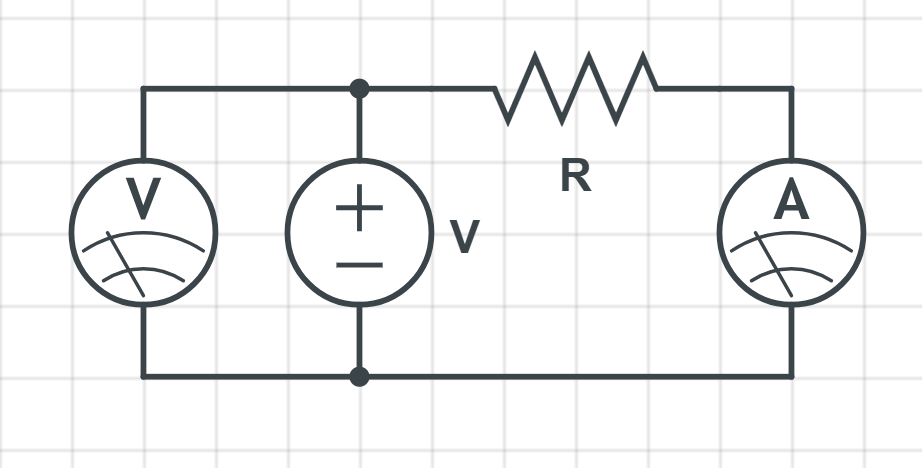
\includegraphics[width=2in]{Ohm}
	\end{center}
	\caption{Depiction of Method of Measuring Current and Voltage}
\end{figure}
In order to verify that the relationship between voltage and current are indeed linear one may measure the current at through a resistor at various different voltages. A variable power supply was attached to a fixed resistor. The current through the resistor was measured with a digital ammeter connected in series with the resistor. The voltage drop across the power supply was also measured with a digital voltmeter. The variable power supply initially provided a potential difference of 0 V, this voltage was gradually increased from 0 V to 5 V over the course of about 50 seconds. The voltage was then decreased gradually from 5 V to 0 V over the course of another 50 s. Throughout the process, 3 data points (current and voltage) were collected every other second.
A light bulb was used instead of a fixed resistance resistor for model a \textit{non-ohmic} resistor. The bulb was positioned in the place where the resistor had been previously, and the voltage was slowly raised from 0 V. In order to avoid damaging the bulb, it was only raised to approximately 2.5 V.
\subsection{Data}
The procedure above was used to collect about 180 data points for each of the resistors and bulbs. Examining these shows that at least for 2 of the resistors the data seems extraordinarily linear. In fact, for the resistors with resistance 555 \( \Omega \) and 2.63 k\(  \Omega \) the correlations for a linear fit are 0.998 and 0.997 respectively. Both also seem to be close to a proportional fit as well, that is, when the the voltage is zero the current seems to be zero as well. Examining the linear regression confirms this, the y-intercepts of the graphs are \( -8 * 10^{-5} \pm 2 * 10^{-5} \) A and \( -9 * 10^{-5} \pm 5 * 10^{-5} \) A respectively. This small deviation may be explained by a slight miscalibration in the current measuring probe.

The data for the other two schemes is not nearly as nice. For the largest resistor (4.68 k\( \Omega\)) the current measured for voltages under 1.5 V fluctuated wildly. Perhaps because the current was so small (under 0.3 mA) the current probe was not able to accurately measure the current through the resistor. However, this range did not prove to be a major issue for the second resistor which also briefly included very small currents. After this point the data proved to be linear.

The bulb, as predicted was \textit{non-ohmic}, the currents measured did not related proportionally with the voltage rather, the rate at which current increased decreased as voltage increase.

For the resistors, the slopes of the graphs and their inverses may be used to compute the overall resistance
\begin{figure}[h]
	\centering
\begin{tabular}{r|c|c}
	Resistor & Slope (\( \Omega^{-1} \)) & Resistance (\( \Omega \)) \\
	555 \( \pm 2 \Omega \) & \(1.834 * 10^{-3} \pm 8 * 10^{-6} \; \Omega^{-1} \)&   \( 545 \pm 2 \; \Omega \)  \\
	2.63 \( \pm 0.2 k\Omega \) &  \(3.76 * 10^{-4} \pm 2 * 10^{-6} \; \Omega^{-1} \) & \( 2.66 \pm 0.01 \; k\Omega \)  \\
	4.68 \( \pm 0.2 k\Omega \) &  \(1.94 * 10^{-4} \pm 7 * 10^{-6} \; \Omega^{-1} \) & \( 5.1 \pm .2 \; k\Omega \)
\end{tabular}
\end{figure}
\begin{figure}
	\centering
	\begin{tikzpicture}
	\begin{axis}[
		align=center,
		title style={yshift=1.5ex},
		title = Current through Resistor (555 \( \mathrm{\Omega} \) ) \\ at variable voltage,
		width = 3 in, height = 3 in,
		xlabel = Voltage (\(V\)), ylabel = Current (\(A\)),
		grid=both,
		minor tick num=5,
		grid style={line width=.1pt, draw=gray!10},
		major grid style={line width=.2pt,draw=gray!50}]
		\addplot[mark = *, mark size = 1, color = blue] table [scatter, only marks, x = res1v, y = res1i, col sep=comma] {data2.csv};
		\addplot[red,samples=111,domain=0:5,thick] {0.001834*x-0.0000845};
	\end{axis}
\end{tikzpicture}
\begin{tikzpicture}
\begin{axis}[
align=center,
title style={yshift=1.5ex},
title = Current through Resistor (2.63 \( \mathrm{k\Omega} \) ) \\ at variable voltage,
width = 3 in, height = 3 in,
xlabel = Voltage (\(V\)), ylabel = Current (\(A\)),
grid=both,
minor tick num=5,
grid style={line width=.1pt, draw=gray!10},
major grid style={line width=.2pt,draw=gray!50}]

\addplot[mark = *, mark size = 1, color = blue] table [scatter, only marks, x = res2v, y = res2i, col sep=comma] {data2.csv};
\addplot[red,samples=111,domain=0:5,thick] {0.000376*x-0.0000987};
\end{axis}
\end{tikzpicture}
\end{figure}
\begin{figure}
	
	\begin{tikzpicture}
	\begin{axis}[
	align=center,
	title style={yshift=1.5ex},
	title = Current through Resistor (4.68 \( \mathrm{k\Omega} \) ) \\ at variable voltage,
	width = 3 in, height = 3 in,
	xlabel = Voltage (\(V\)), ylabel = Current (\(A\)),
	grid=both,
	minor tick num=5,
	grid style={line width=.1pt, draw=gray!10},
	major grid style={line width=.2pt,draw=gray!50}]
	\addplot[mark = *, mark size = 1, color = blue] table [scatter, only marks, x = res3v, y = res3i, col sep=comma] {data2.csv};
	\addplot[red,samples=111,domain=0:5,thick] {0.0001942*x-0.00000059};
	\end{axis}
	\end{tikzpicture}
	\begin{tikzpicture}
	\begin{axis}[
	align=center,
	title style={yshift=1.5ex},
	title = Current through Bulb \\ at variable voltage,
	width = 3 in, height = 3 in,
	xlabel = Voltage (\(V\)), ylabel = Current (\(A\)),
	grid=both,
	minor tick num=5,
	grid style={line width=.1pt, draw=gray!10},
	major grid style={line width=.2pt,draw=gray!50}]
	
	\addplot[mark = *, mark size = 1, color = blue] table [scatter, only marks, x = liv, y = lii, col sep=comma] {data2.csv};
	\addplot[red,samples=111,domain=0:2.5,thick] {(-.1376273053+.8821538213e-1*sqrt((14.532*x*x+2.434)))/x};
	\end{axis}
	\end{tikzpicture}
\end{figure}
\subsection{Analysis}
Ohm's Law, \( V = I R\) effectively models the current-voltage relationship for the purpose built resistors. However, being \textit{non-ohmic}, the bulb is more difficult to model. Ultimately the non-linearity of the bulb's curve stems from its constant change in temperature. A change in temperature brings about a change in resistance. For most materials this means an increase in temperature will result in an increase in resistance. Typically this relationship is described as 
\begin{equation}
R = R_0 (1 + \alpha(T-T_0))
\end{equation}
where \(T\) is temperature and \(\alpha\) is some proportionality constant called the temperature coefficient of resistance.

One might assume that the increase in temperature of the bulb is proportional to its power. The power dissipated by the bulb is 
\begin{equation}
P \propto I^2 R
\end{equation}
This means that the resistance should be expressible as
\begin{equation}
R = R_0 (1 + \alpha \, I^2 \, R)
\end{equation}
It is convenient to solve for current in terms of voltage rather than resistance. Thus we may subsistent \(R\) for \(V/I\).
\begin{equation}
\frac{V}{I} = R_0 (1 + \alpha \, V \, I)
\end{equation}
Solving for current yields the somewhat clunky expression
\begin{equation}
I = \frac{-R_0 + \sqrt{4\,R_0\, \alpha \, V^2 + R_0^2}}{2\, R_0 \, \alpha \, V}
\end{equation}
This should match the data collected for the bulb, however the fit seems quite disappointing. It generally captures the trend of graph but seems to curve more than the true data. The coefficients are found to be

\[R_0 = 2.42 \pm 0.6 \Omega \]

\[\alpha = 3.6 \pm 0.2 \; C^{-1} \]

\subsection{Conclusions}
The three resistors measured followed the trend of Ohm's law incredibly well. The current related to voltage in a linear relation. The resistances calculated using the linear fit to the data come relatively close to the measured resistances for each of the resistors. Resistor 1 was measured to be \(555 \pm 2 \Omega \) while the linear fit predicted it to be \(545 \pm 2 \Omega \). This constitutes an error of about 1.8 \%. The second resistor had similarly good results. It  was measured to be \( 2.63 \pm 0.02 \; k \Omega \) while the data suggested a more appropriated value of  \( 2.66 \pm 0.02 \,k  \Omega \), constituting an error of closer to 1.1\%. While these values are quite close to their expected values, the third resistor is much farther off, measured at \( 4.68 \pm 0.02 \; k \Omega \) while the data would suggest that the resistance is closer to \( 5.1 \pm 0.2 \; k \Omega \) is error is a much larger 8.9\%. Part of the increased error in resistor 3 may be explained by the issues with current measurement. While the other issues in measurement that account for the 1 - 2 \% error in the others may be explained by some small internal resistance in the ammeter, some small amounts of current passing through the voltmeter and other issues in measurement.

The fit of the curve on the bulb is somewhat more troubling, however some of its short comings may be explained by the model. The model used for the fit assumes that the temperature of the bulb is directly proportional to the power dissipated. This is a naive interpretation as the bulb will of course have some sort of thermal inertia. That is, the bulb will take time to reach its stable temperature at any given voltage, however the voltage was changed rather rapidly and the bulb was not given sufficient time to adjust after each change in voltage.

The parameters for the fit have some meaning as well.\(R_0\) is meant to represent the resistance of the bulb at room temperature. This would imply that the resistance of the bulb at this temperature is \(  2.42 \pm 0.6 \Omega \). This value seems to agree visually with the inverse slope of the current voltage curve around zero which appears to be in the 2.5-3 \(\Omega\) range. The calculated 2.42 value does not fall within this range bt has a very broad uncertainty which certainty pushes the value into this range. The \( \alpha \) parameter was meant to represent the temperature coefficient of the  material, however one might notice that \(3.6 \pm 0.2 \; C^{-1} \) is nowhere near the temperature coefficient of tungsten, \( 0.0044 C^{-1}\) \footnote{https://www.allaboutcircuits.com/textbook/direct-current/chpt-12/temperature-coefficient-resistance/}
However, this was based on the naive assumption that one Watt of power would result in a degree increase in temperature, this is simply not the case. Instead, alpha is the product of the temperature coefficient of tungsten and the ratio of watt power to degree Celsius. Dividing \(  \alpha\) by the temperature coefficient of tungsten should yield the amount of power required to increase the temperature of the resistor by one degree Celsius. This value is \(810 \pm 50 W/C\)

\section{Kirchoff's Laws}

\subsection{Introduction}
	Kirchoff's Laws are a series of equabilities that describe the distribution of current and electric potential within a circuit. Essentially they state that the voltage across any closed loop is 0, and that the current through any junction is 0. One may use these principles to determine the resistance, current, and voltage of any given circuit. For example, consider 3 resistors in series, \(R_1,R_2,R_3\) and an ideal voltage source \(V\). Because the current through a closed loop must be equal to 0, we know that the equality \( V - I R_1 - I R_2 - I R_3 = 0\) must hold. This may be factored to show that \(V - I(R_1+R_2+R_3) \). This shows that resistors effectively add in series. Similarly consider two resistors \(R_1, R_2\)  attached in parallel to an ideal voltage source \(V\). Because currents must sum to zero in a junction \begin{equation}
	\frac{V}{R} = \frac{V}{R_1} + \frac{V}{R_2}.
	\end{equation}This shows that in parallel resistors are the inverse of the sum of the inverses. \begin{equation} \frac{1}{R} = \frac{1}{R_1} + \frac{1}{R_2}. \end{equation}
\subsection{Procedure}
	In order to demonstrate that Kirchoff's laws do in fact hold a series of circuits were arranged and the currents, voltages and resistances were measured at a variety of points. Three resistors, 555, 2630 and 4680 \( \Omega\) were arranged in three separate schemes. First they were arranged in series, then all in parallel, and eventually in a combined scheme were resistors were both in series and in parallel. These were all connected to a 5 V ideal voltage supply. The three arrangements are pictured below.
\begin{figure}[h]
	\begin{center}
		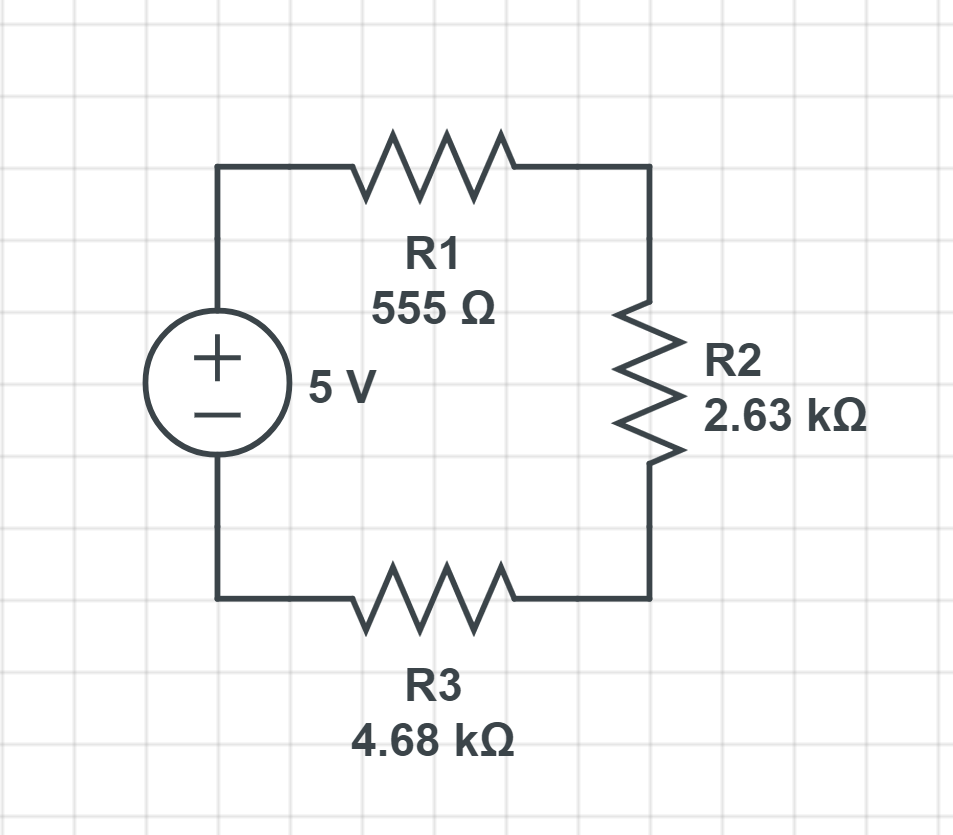
\includegraphics[scale=0.3]{S1}
		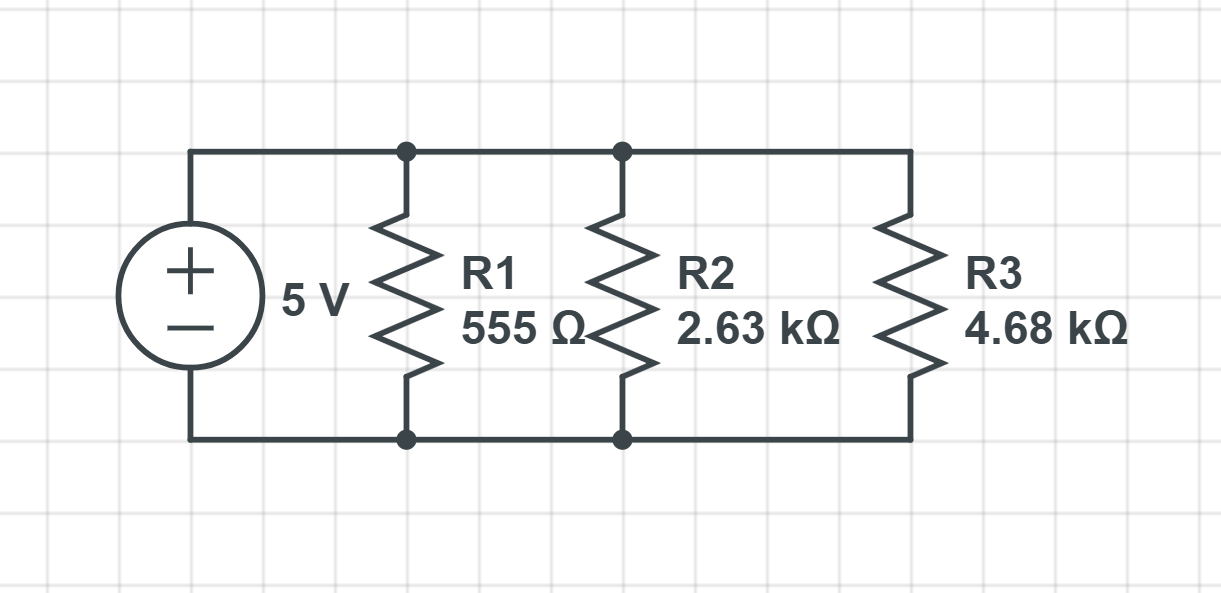
\includegraphics[scale=0.3]{S2}
		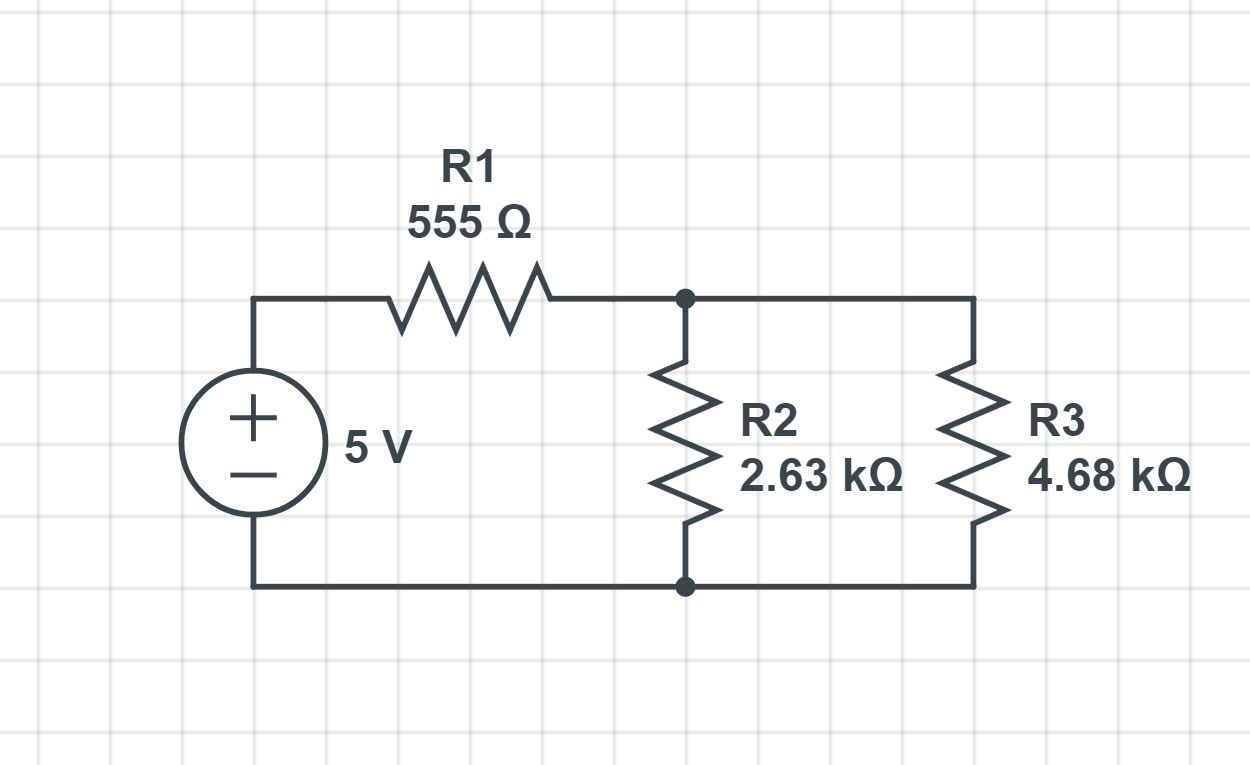
\includegraphics[scale=0.3]{S3}
	\end{center}
\end{figure}
\subsection{Data}
The voltage current and resistance were measured for each circuit.
\begin{figure}[h]
	\centering
	\caption{Measurements of Series Circuit} 
	\begin{tabular}{|c|c|c|c| }
		\hline
		Location & Resistance  k\(\Omega\) & Current (mA) & Voltage (V) \\ \hline
		\(R_1\) & 0.555 & 6.38 & 0.357 \\
		\(R_2\) & 2.63 & 6.38 & 1.69 \\
		\(R_3\) & 4.68 & 6.38 & 3.03 \\
		Total & 7.92 & 6.38 & 5.07 \\
		\hline
	\end{tabular}

\end{figure}
\begin{figure}[h]
	\centering
	\caption{Measurements of Parallel Circuit} 
	\begin{tabular}{|c|c|c|c| }
		\hline
		Location & Resistance  k\(\Omega\) & Current (mA) & Voltage (V) \\ \hline
		\(R_1\) & 0.555 & 8.97 & 5.07 \\
		\(R_2\) & 2.63 & 1.862 & 5.07 \\
		\(R_3\) & 4.68 & 1.057 & 5.07 \\
		Total & 0.419 & 11.85 & 5.07 \\
		\hline
	\end{tabular}
	
\end{figure}
\begin{figure}[h]
	\centering
	\caption{Measurements of Combined Circuit} 
	\begin{tabular}{|c|c|c|c| }
		\hline
		Location & Resistance  k\(\Omega\) & Current (mA) & Voltage (V) \\ \hline
		\(R_1\) & 0.555 & 2.24 & 1.254 \\
		\(R_2\) & 2.63 & 1.140 & 3.81 \\
		\(R_3\) & 4.68 & 0.795 & 3.81 \\
		Total  & 2.27 & 2.24 & 5.07 \\
		\hline
	\end{tabular}
\end{figure}
\\
The resistances under 2000 \(  \Omega \) are measured to the nearest 2 \( \Omega \) while those above 2000 are measured to the nearest  20 \( \Omega \). Currents are accurate within 0.5 \% of the stated value. Voltages under 2 V measure to the nearest millivolt while those above 2 V are accurate the the nearest 10 \( mV \).
\subsection{Analysis}
\subsubsection{Series Circuits}
Kirchoff's Laws make several statements about properties that should hold in a series circuit. The most obvious of switch is simply the loop rule, that is, the voltages through each of the resistors should sum to the voltage drop across the power supply. Simply put
\begin{equation}
V = V_1 + V_2 + V_3.
\end{equation}
One may extend this notion to the resistances as was done in the introduction. Alternatively, the effective resistance across the circuit is equal to the sum of the sub resistors.

\begin{equation}
R = R_1 + R_2 + R_3.
\end{equation}
Because there exist no junctions in the circuit the current through each of the components should remain constant.
\subsubsection{Parallel Circuits}
In a parallel circuit voltages should be constant as each of the components form their own loop with the voltages source.  This may be expressed as 
\begin{equation}
V = V_1 = V_2 = V_3.
\end{equation}
Each of these voltages should be equal to the product of the current through the circuit and the resistance.

In parallel, resistances sum as the inverse of the sum of the inverses, this is simply a  corollary of the loop rule and Ohm's law.
\begin{equation}
R = \frac{1}{ \frac{1}{R_1} + \frac{1}{R_2} + \frac{1}{R_3}  }
\end{equation}

From these one may deduce the currents through each of the 3 resistors. By Ohm's law the current through a resistor with a resistance \(R\) and voltage \(V\) is a \(V / R \). 
\begin{equation}
I_1 = \frac{V}{R_1},I_2 = \frac{V}{R_2},I_3 = \frac{V}{R_3}
\end{equation}
\subsubsection{Combined Circuit}
This circuit is a little bit more complicated than the previous two. 

Being in parallel, the voltages through \(R_2\) and \(R_3\) should be equal and these should sum with \(V_1\) to get the sum \(V\).

\begin{equation}
V = V_1 + V_2 = V_1 + V_3
\end{equation}

The overall resistances are summed both as in series and as in parallel. 

\begin{equation}
R = R_1 + \frac{1}{\frac{1}{R_2}+\frac{1}{R_3}}
\end{equation}

The junction present in the circuit should obey Kirchoff's junction rule.

\begin{equation}
I = I_1 = I_2 + I_3
\end{equation}
\subsection{Conclusions}
All of the rules in the above section are obeyed by the three circuits.
\subsubsection{Series Circuit} 
\paragraph{Resistance}
In a series circuit the resistances sum to give a single effective resistance. Summing the measured resistances yield a effective resistance of \(  7.87 \pm 0.03 \mathrm{ k \Omega } \). This summed value is just under the measured total resistance  \( 7.92 \pm 0.02 \mathrm{ k \Omega }\). These values are just within each others uncertainty and have a total difference of 0.7 \%.
\paragraph{Current} Having computed the overall total resistance and measured the voltage though the power supply one may find the current through the whole system. Dividing the measured voltage by the calculated resistance yields a calculated current of \( 6.44 \pm 3\) mA. This is under measured current of \(6.38 \pm 0.03\) mA and off by about 0.9\%. This current should and did remain constant across the whole circuit.
\paragraph{Voltage}
The voltage drop through each resistor should be equal to the current though the resistor multiplied by its resistance. The calculated voltages are \(0.355 \pm 0.02\) V, \(1.69 \pm 0.02\) V, and \( 3.01 \pm 0.02 \) V. These are remarkably close to the measured voltages. In fact, 2 of these values are the exact voltages measured. The only one that is off is the third voltage which is of by a mere 0.6 \%. These voltages sum to \(5.06 \pm 0.03\) V. This is an error of merely 0.2\%. This confirms Kirchoff's law.
\subsubsection{Parallel Circuit} 
\paragraph{Resistance}
In a parallel circuit, the resistances sum as the inverse of the sum of the inverses. The total effective resistance is computed to be \(417 \pm 2 \Omega\). This is within 0.5 \% of the measured value.
\paragraph{Current}
One may use Ohm's law to compute the ideal currents across each of the resistors. This calculation shows that the currents through each of the resistors should be \(9.14 \pm 0.05 \) mA, \(1.93 \pm 0.02 \) mA, \(1.083 \pm 0.007 \) mA. These are generally good estimates but represent a overestimation of the measured currents by 1.9\%, 3.6\%, and 2.7\%.

\paragraph{Voltage}
In parallel, voltage is equal, thus it makes sense that all measured voltages were the same as the total voltage measured. 

\subsubsection{Combined Circuit} 
\paragraph{Resistance}
In this combined circuit, the effective total resistance may be found by combining the methods for parallel and series circuits. Doing this will yield an calculated effective resistance of \( 2.24 \pm 0.01 \) k\(\Omega\). This is 1.3 \% below the measured value of \( 2.27\) k\(\Omega\).
\paragraph{Current}
The current through the first resistor should be the same as the current through the whole system. Thus one can find this simply using Ohm's law. This calculation would conclude the current though the system to be \(2.26 \pm 0.01 \) mA, 0.9\% higher than the measured value of \(2.24\)mA. The other two currents should sum to get this previous current (Loop Rule) and should also be inversely proportional to the resistance through the resistors (Ohm's Law). This rules may be rearranged to say that 
\begin{equation}
I_2 = \frac{I R_3}{R_2 + R_3}, \text{  } I_3 = \frac{I R_2}{R_2 + R_3}
\end{equation}
These equations predict the currents through the resistors to be \(1.447 \pm 0.008\) mA and \(0.813 \pm 0.006\)mA. The later of these values is an overestimation of 2.2\%. But the first value is more troubling. Taken as written these predict an error of over 25\%. This is troubling and doest fit well with the other data taken. It is possible and very likely that some kind of error in transcription occurred and the measured value was perhaps 1.410 mA or 1.440 mA which would better fit with the remaining data. However, the original manuscript is no longer in the possession of the author who can do no better than guess at the true value. These guessed values provide errors of 2.5\%  (for 1.410 mA) or  0.3\% for (1.440 mA). The previous errors indicate that 1.410 is the most likely answer.
\paragraph{Voltage} With calculated currents and measured resistances one need only take a product to find the voltages across each resistor. One should expect the second two voltages to be the same.
The first voltage was found to be \( 1.254 \pm 0.07 \) V, exactly the measured voltage. The second was found to be \(3.81 \pm 0.04\) V, also exceptionally close to the measured voltage. The third and final was found to be \(3.81 \pm 0.05\) V, like the other 3 accurate to within the significant figures of the measurement.
\subsubsection{General Conclusions}
The measurements gathered here agreed with both Kirchoff's laws and with Ohm's law. All values  predicted were exceptionally close to their measured values, and the variability apparent is rather easily explained. Resistance was consistently underestimated, this means that there is some agent acting to increase the resistance of the system without our knowledge. This stems from the fact that the voltages source, resistance probe, and wires have some small unaccounted for resistance. The underestimation in resistance accounts for the constant over estimation in current. Voltage was consistently accurate.
\end{document}